% Scalar instruction entry source: tools/generate_scalar_instruction_catalog.py.
\subsection{\texttt{JAL}}
\label{sec:scalar-jal}
\index{JAL@\texttt{JAL}}
\begin{sloppypar}\noindent\textbf{Purpose.} Writes the return address to Ra and transfers control to the PC-relative target.\end{sloppypar}\smallskip
\noindent\textbf{Syntax.}\par
\begin{lstlisting}[style=ptoscalarcode]
jal simm, ->Ra
\end{lstlisting}
\noindent\textbf{Encoding.}\par
\noindent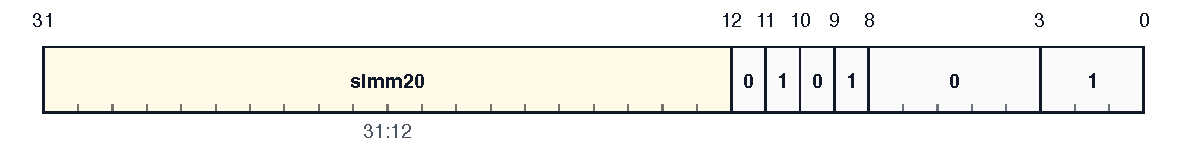
\includegraphics[width=\textwidth]{figs/encoding/scalar_instruction_entries/enc_jal.pdf}\par\smallskip
\begin{description}[leftmargin=0.18\linewidth,style=nextline]
\item[Format] \texttt{L32} \texttt{32-bit} scalar word.
\item[Pattern] \texttt{....................010100000111}.
\end{description}
\noindent\textbf{Classification.}\par
\begin{description}[leftmargin=0.18\linewidth,style=nextline]
\item[Category] Branch, Compare, and PC Control.
\item[Family] PC-Relative.
\item[Execution class] \texttt{BRU}; uop\_kind=BRU.
\end{description}
\noindent\textbf{Operand fields.}\par
\begin{description}[leftmargin=0.18\linewidth,style=nextline]
\item[\texttt{simm20}] Bits \texttt{31:12 (20b)}. 20-bit signed PC-relative displacement used to form the jump or address result.
\end{description}
\noindent\textbf{Operation.}\par
\begin{lstlisting}[style=ptoscalarcode]
base = CurrentPC()
off = (ZeroExtend(imm20) << 1)
ra = base + off
\end{lstlisting}
\Needspace{0.08\textheight}
